\section{Wielomiany Czebyszewa (Chebyshev Polynomials)}
%%%%%%%%%%%%%%%%%%%
\begin{frame}{Reprezentacja trygonometryczna}
	$$\cos(n\varphi)+\cos[(n-2)\varphi] = 2\cos[(n-1)\varphi] \cdot \cos \varphi$$
    $$\cos(n\varphi) = 2\cos[(n-1)\varphi] \cdot \cos \varphi - \cos[(n-2)\varphi]$$
    dla $x \in [-1,1]\Rightarrow \varphi=\arccos x$
    $$T_n(x) = \cos[n \cdot \arccos x]$$
\end{frame}
%%%%%%%%%%%%%%%%%%%
\begin{frame}{Relacja rekurencyjna}
	\begin{tabular}{l}
		$T_0(x) = 1$ \\
        $T_1(x) = x$ \\
        $T_2(x) = 2x^2-1$ \\
        $T_3(x) = 4x^3-3$ \\
        $T_4(x) = 8x^4-8x^2+1$ \\
        $T_5(x) = 16x^5-20x^3+x+3\ldots$ \\
        $\vdots$ \\
        $T_n(X) = 2xT_{n-1}(x) - T_{n-2}(x)$
	\end{tabular}
    
    \begin{block}{Czynnik wiodący}
    	Czynnik wiodący w $T_n(x)$ jest to czynnik przy najwyższej potędze $x$ : $2^{n-1}$
    \end{block}
\end{frame}
%%%%%%%%%%%%%%%%%%%
\begin{frame}{Symetria}
	$$T_k(-x)=(-1)^k \cdot T_k(x)$$
    \begin{figure}
		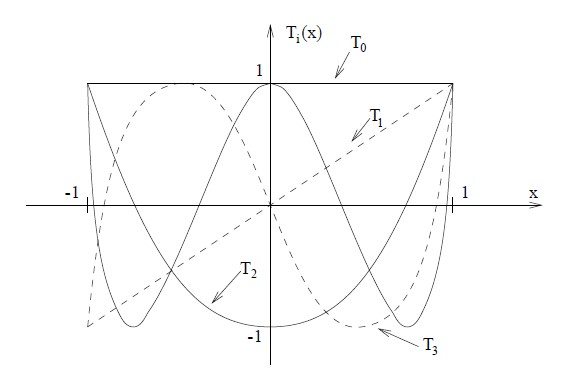
\includegraphics[height=0.75\textheight]{img/5/symetria.jpg}
	\end{figure}
\end{frame}
%%%%%%%%%%%%%%%%%%%
\begin{frame}{Zera $T_n(x)$ - węzły Czebyszewa}
	$T_n(x)$ ma w $[-1,1]$ $n$ zer:\newline
    $x_k = \cos (\frac{2k+1}{n} \cdot \frac{\pi}{2}), k=0,1,..,n-1$
    $$T_n(x) = \cos(n \underbrace{\arccos x}_\alpha)$$
    $$\cos(n \cdot \alpha) = 0 \text{ dla } n \cdot \alpha = (2k+1) \cdot \frac{\pi}{2},k=0,1,..,n-1$$
\end{frame}
%%%%%%%%%%%%%%%%%%%
\begin{frame}{Ortogonalność}
	\begin{block}{Przypadek ciągły}
		$$\int_{-1}^{1}\frac{T_i(x) \cdot T_j(X)}{\sqrt{1-x^2}}dx = \left\{\begin{array}{lc}
			0 & i \not= j \\
            \frac{\pi}{2} & i = j \not= 0 \\
            \pi & i = j = 0 \rightarrow \text{repr. tryg.}
		\end{array}\right.$$
	\end{block}
    
    \begin{block}{Przypadek dyskretny $x_k = $ Zera $[T_{m+1}(x)]$}
    $$\sum_{k=0}^{m}T_i(x_k)T_j(x_k) = \left\{\begin{array}{rc}
    	0 & i \not= j \\
        \frac{m+1}{2} & i=j \not= 0 \\
        m+1 & i=j=0
    \end{array}\right.$$
    \end{block}
\end{frame}
%%%%%%%%%%%%%%%%%%%
\begin{frame}{Własność minimaksu wielomianów Czebyszewa}
	\begin{block}{Twierdzenie o normie $T_n(x)$}
		Ze wszystkich wielomianów stopnia $n$ z czynnikiem wiodącym równym 1 najmniejszą normę maksymalną w $[-1,1]$ 
        $$\lVert W_n \rVert _{\infty} = max_{x \in [a,b]}|W_n|$$
        ma wielomian $2^{1-n} \cdot T_n(x)$. Wynosi ona $2^{1-n}$
	\end{block}
\end{frame}
%%%%%%%%%%%%%%%%%%%
\begin{frame}
	\textbf{Dowód (nie wprost) }\newline
	\begin{tabular}{|l}
		Załóżmy, że $\exists p_n(x)$ o współczynniku wiodącym = 1 taki, że:
      \\$\forall_{x \in [-1,1]}|p_n(x)| < 2^{1-n}$ wszystkie $T_n(1) = 1$, $x = 1$\\ $\Rightarrow x_0'$ (punkt ekstremalny) \\
	\end{tabular}	
    \begin{figure}
		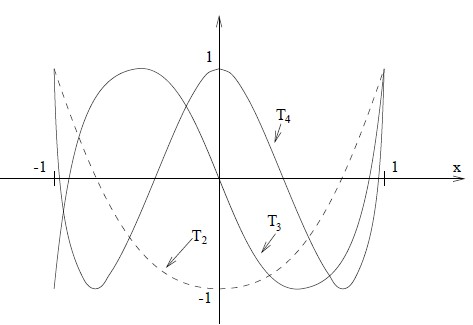
\includegraphics[height=0.7\textheight]{img/5/dowod.jpg}
	\end{figure}
\end{frame}
%%%%%%%%%%%%%%%%%%%
\begin{frame}
	\begin{tabular}{|l}
		Odcięta punktu ekstremalnego $T_n(x)$, $x_k'=\cos\frac{k\pi}{n}$, $k=0,1,..,n$\\
        Dla $\forall x_k'$ powinno zachodzić: \\
        $p_n(x_0') < 2^{1-n} \cdot T_n(x_0')$, \\
        $p_n(x_1') > 2^{1-n} \cdot T_n(x_1')$, \\
        $p_n(x_2') < 2^{1-n} \cdot T_n(x_2')$, \\
        \ldots , aż do $x_n'$ \\
        $\Rightarrow$ czyli wielomian $[p_n(x) - 2^{1-n} \cdot T_n(x)]$ \\
        powinien zmieniać znak w każdym z przedziałów: \\
        $(x_{k+1}',x_k')$, $k = \underbrace{n-1, n-2,..,1,0}_{\text{n przedziałów $\rightarrow$ n zer}} $\\ 
         $\Rightarrow $ czyli powinien być wielomianem stopnia $n$ w $[-1,1]$, \\ 
         ale $p_n(x)$ i $2^{1-n} \cdot T_n(x)$ mają ten sam współczynnik wiodący, \\
         Zatem ich różnica jest stopnia $n-1$ i mamy sprzeczność!!!
	\end{tabular}
\end{frame}
%%%%%%%%%%%%%%%%%%%
\begin{frame}{Aproksymacja wielomianami Czebyszewa}
	$\rightarrow$ jednostajna: $min!sup_{x \in [a,b]}|F(x)-f(x)|$ \newline
    baza $T_i(x)$ wygodna, bo $T_i(x)$ - równomierne w $[-1,1]$ \newline
    $F(x)$ \textbf{zastępujemy sumą częściową:}
    $$F(x) \approx \sum_{j=0}^{N}c_jT_j(x)$$
    z $c_j$ wyznaczonymi z warunku ortogonalności w przypadku ciągłym
    $$F(x) = \sum_{j=0}^{\infty}c_jT_j(x)\bigg\arrowvert \frac{T_i(x)}{\sqrt{1-x^2}},\int_{-1}^{1}dx$$
    \begin{tabular}{ll}
    $c_0 = \frac{1}{\pi}\int_{-1}^{1}\frac{F(x)dx}{\sqrt{1-x^2}}$ &
    $c_i = \frac{2}{\pi}\int_{-1}^{1}\frac{F(x)dx}{\sqrt{1-x^2}}, i=1,..,N$
    \end{tabular}
    
    Często - zamiast $\uparrow \rightarrow$ interpolacja $T_{n+1}(x)$
\end{frame}
%%%%%%%%%%%%%%%%%%%
\begin{frame}
	\textbf{Tworzymy wyrażenia wymierne postaci:}
    $$T_{n,k}(x) = \frac{\sum_{i=0}^{n}a_iT_i(x)}{\sum_{i=0}^{k}b_iT_i(x)}$$
    o $a_i$, $b_i$ dobranych tak, by w liczniku wyrażenia 
    $$F(x)-T_{n,k}(x) = \frac{\big[\sum_{j=0}^{\infty}c_jT_j(x)\big] \cdot \big[\sum_{i=0}^{k}b_iT_i(x)\big] - \sum_{i=0}^{n}a_iT_i(x)}{\sum_{i=0}^{k}b_iT_i(x)}$$
    znikały współczynniki dla $T_i(x),i=0,1,2,..,k+n$
\end{frame}
%%%%%%%%%%%%%%%%%%%
\begin{frame}{Interpolacja Czebyszewa (z węzłami $T_{n+1}(x)$)}
	$W_n(x)$ - wielomian interpolacyjny stopnia $n$; $W_n(x) = f(x_k),k=0,1,..,n$
    $$f(x) = W_n(x)+E_n(x); E_n(x) = \frac{f^{(n+1)}(c)}{(n+1)!}\underbrace{\prod_{i=0}^{n}(x-x_i)}_{\omega_n}
	, c \in [x_0,x_n]$$
    Przez optymalny wybór rozmieszczenia węzłów $x_k \rightarrow$ zminimalizować $max|\omega_n(x)|$\newline
    $\Rightarrow$ \textbf{Rozwiązanie:} Wprost z własności minimaksu $T_{n+1}(x)$ jako $x_k$ wziąć węzły - zera $T_{n+1}(x)$:
    $$x_k = \cos \Big(\frac{2k+1}{n+1}\pi\Big), k=0,1,..,n \rightarrow \text{interpolacja Czebyszewa}$$
    
\end{frame}
%%%%%%%%%%%%%%%%%%%
\begin{frame}
	- interpolacja z równoodległymi węzłami (11 węzłów)\newline
    - interpolacja z węzłami Czebyszewa $\rightarrow$ zera $T_{11}(x)$
    \begin{block}{Uwaga}
    Transformacja przedziału $x \in [a,b] \rightarrow t \in [-1,1]$
    $$x=\frac{b-a}{2}t+\frac{a+b}{2}$$
    \end{block}
\end{frame}
%%%%%%%%%%%%%%%%%%%
\begin{frame}
	\begin{figure}
		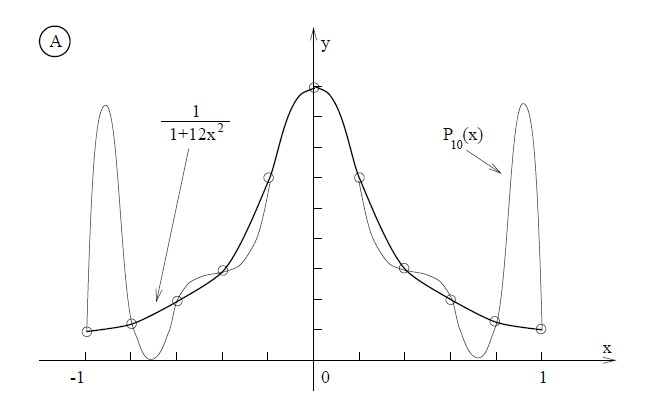
\includegraphics[height=0.8\textheight]{img/5/czebyszew.jpg}
	\end{figure}
\end{frame}
%%%%%%%%%%%%%%%%%%%
\begin{frame}{Interpolujący wielomian Czebyszewa}
	$T_n(x)$ zachowują się równomiernie w $[-1,1]$; min = -1, max = 1 - \textbf{ważna własność} \newline
    Do utworzenia wielomianu interpolacyjnego używamy liniowej kombinacji:
    $$W_n(x) = \sum_{j=0}^{N}c_jT_j(x)$$
    $\{c_j\}$ - z własności ortogonalności dla przypadku dyskretnego:
    $$x_k=\cos\Big(\frac{2k+1}{N+1}\frac{\pi}{2}\Big)\rightarrow \text{zera } T_{N+1}(x),k=0,1,..,N$$
    $$\sum_{k=0}^{N}T_i(x_k)T_j(x_k) = \left\{\begin{array}{cc}
    	0 & i \not= j \\
        N+1 & i=j=0 \\
        \frac{N+1}{2} & i=j\not=0
    \end{array}\right.$$
\end{frame}
%%%%%%%%%%%%%%%%%%%
\begin{frame}{Warunek interpolacji}
	$$f(x_k)= \sum_{j=0}^{N}c_jT_j(x_k)\Bigg\arrowvert T_i(x_k),\sum_{k=0}^{N}$$
    $$\sum_{k=0}^{N}f(x_k)T_i(x_k)=\sum_{j=0}^{N}c_j\underbrace{\sum_{k=0}^{N}T_i(x_k)T_j(x_k)}_{\text{ortogonalność}}$$
\end{frame}
%%%%%%%%%%%%%%%%%%%
\begin{frame}
	\begin{figure}
		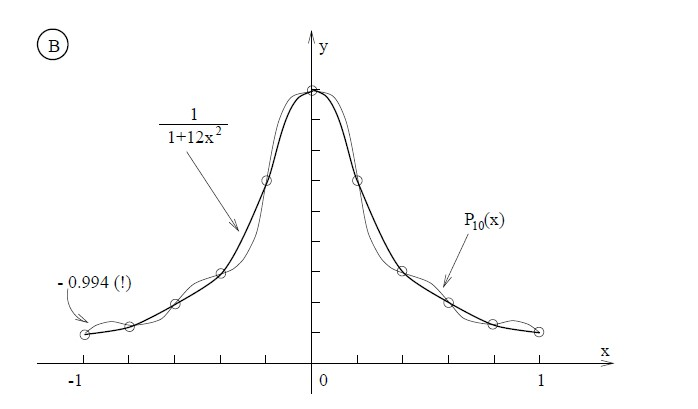
\includegraphics[height=0.8\textheight]{img/5/interpolacja.jpg}
	\end{figure}
\end{frame}
\begin{frame}{Współczynniki $c_i$}
	$$c_0 = \frac{1}{N+1}\sum_{k=0}^{N}f(x_k)T_0(x)=1$$
    $$c_i = \frac{2}{N+1}\sum_{k=0}^{N}f(x_k)T_i(x_k)$$
    Pozostaje nam wyliczenie sumy.
\end{frame}
%%%%%%%%%%%%%%%%%%%
